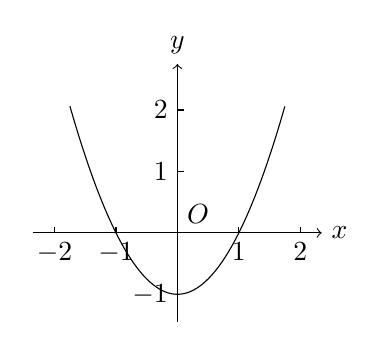
\begin{tikzpicture}[x=.78cm,y=.78cm,baseline=(current bounding box.center)]
  \draw[->] (-2.35,0)--(2.35,0) node[right] {$x$}; \draw[->] (0,-1.45)--(0,2.75) node[above] {$y$};
  \draw[domain=-1.75:1.75,samples=100,smooth] plot (\x,{\x*\x-1});
  \draw (-2,0)--(-2,.10) (-1,0)--(-1,.10) (1,0)--(1,.10) (2,0)--(2,.10) (0,1)--(.10,1) (0,2)--(.10,2);
  \node[below] at (-2,0) {$-2$}; \node[below] at (-1,0) {$-1$}; \node[below] at (1,0) {$1$}; \node[below] at (2,0) {$2$}; \node[left] at (0,-1) {$-1$}; \node[left] at (0,1) {$1$}; \node[left] at (0,2) {$2$}; \node[above right] at (0,0) {$O$};
\end{tikzpicture}
